\graphicspath{{fig/model_development/}}

\chapter{Model Development}
\label{cha:model_dev}

In this chapter we shall introduce one of the most popular and well studied agent-based
models in the literature: the Vicsek model. The Vicsek model represents a simple alignment
model in which agents interact with neighbours within some given distance. Despite its
simplicity, this model can produce sophisticated dynamics and exhibits a phase
transition from order to disorder as the amount of noise in the system is regulated.

The Vicsek model, like many other ABMs, implements a discontinuous interaction rule. With
this, the onset of interaction between individuals is very sensitive to small
perturbations in distances. We consider continuous interaction rules as a
biologically-motivated alternative. Such rules ensure the model is more robust to small
perturbations in distances, but without the penalty of adding extra model complexity.

\section{The Vicsek Model}

The Vicsek model describes the movements of $N$ individuals moving with constant speed
$v$. All movement takes place in a square-cell with periodic boundary conditions and side
length $L$. To initialise a simulation all agents are allocated a random position within
the cell, and a random direction of motion. From time $t$ to time $t+1$ agent $i$ updates
its position as:
\begin{equation*}
    \bm{x}_{i, t+1} = \bm{x}_{i, t} + \bm{v}_{i, t},
\end{equation*}
where the velocity $\bm{v}_{i,t}$ is constructed to have speed $v$ and direction of motion
$\theta_{i, t+1}$. The computation of $\theta_{i, t+1}$ describes how agents update their
direction in light of their neighbours' movements. The ability of individuals to observe
and react to the movements of their neighbours is assumed to be imperfect, and so a noise
term, in the form of a random directional perturbation, is introduced. In the Vicsek model
noise is considered to be uniformly distributed as $\mathcal{U}(-\eta/2, \eta/2)$. The
directional update of agent $i$ can then be expressed as:
\begin{equation}
    \label{eq:vicsek_update}
    \theta_{i, t+1} \given \angmean{\theta}_{i, t}, \eta \sim
                     \mathcal{U}(\angmean{\theta}_{i, t} - \eta/2,
                                 \angmean{\theta}_{i, t} + \eta/2),
\end{equation}
where $\angmean{\theta}_{i, t}$ represents the average direction of motion of agent $i$'s
neighbours at time $t$. As $\angmean{\theta}_{i, t}$ describes a mean of circular
quantities (directions of motion), its computation necessitates the use of the
circular mean (\cref{eq:atantwo}):
\begin{equation}
    \angmean{\theta}_{i, t+1} = \atantwo\bigg(
        \sum_{j=1}^N \omega_{ij, t} \sin\theta_{j,t},
        \sum_{j=1}^N \omega_{ij, t} \cos\theta_{j,t}
    \bigg).
\end{equation}
With this, $\omega_{ij, t}$ represents the strength of the interaction between agent $i$
and neighbour $j$ at time $t$. In the Vicsek model agent $i$ interacts with neighbours
which are positioned within a circle of radius $r$, which is centered at the position of
agent $i$. This interaction can be implemented with the weighting rule:
\begin{equation}
    \label{eq:vicsek_interaction}
    \omega_{ij,t} =
    \begin{cases}
        1 & \text{ if } d_{ij, t} \leq r,\\
        0 & \text{ otherwise,}
    \end{cases}
\end{equation}
where $d_{ij,t}$ is the Euclidean-distance between the positions of agent $i$ and agent
$j$ at time $t$:
\begin{equation*}
    d_{ij,t} = \sqrt{(x_{j,t} - x_{i,t})^2 + (y_{j,t} - y_{i,t})^2}.
\end{equation*}

The interaction rule implemented in the Vicsek model represents a discontinuous
interaction. We can see this more formally by considering the value of $\omega_{ij, t}$ as
$d_{ij,t}$ tends to $r$ from above and below. As $d_{ij,t}$ tends to $r$ from above we
have that $\lim_{d_{ij,t} \rightarrow r^+} \omega_{ij,t} = 0$. Conversely, we realise a
different value as we consider the limit as $d_{ij,t}$ tends to $r$ from below:
$\lim_{d_{ij,t} \rightarrow r^-} \omega_{ij,t} = 1$.

The Vicsek model was motivated by models for ferromagnetism, and so a discontinuous
interaction may be appropriate for this use-case. However, it is not clear whether the
hard cut-off imposed by the interaction radius is appropriate for biological systems.

\begin{figure}[tb]
    \begin{subfigure}[b]{0.5\textwidth}
        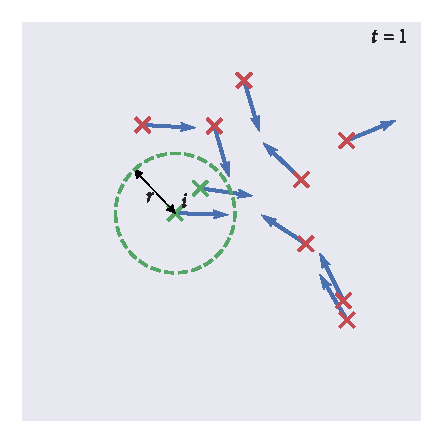
\includegraphics{vicsek_simulation_1.pdf}
    \end{subfigure}%
    \begin{subfigure}[b]{0.5\textwidth}
        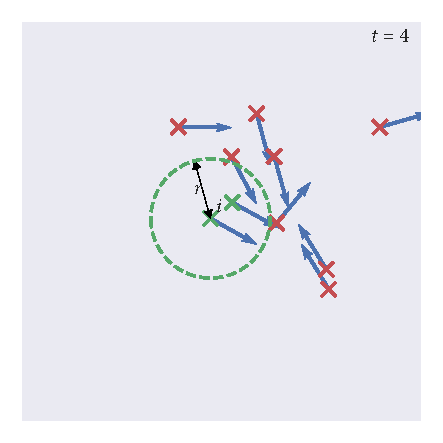
\includegraphics{vicsek_simulation_4.pdf}
    \end{subfigure}
    \begin{subfigure}[b]{0.5\textwidth}
        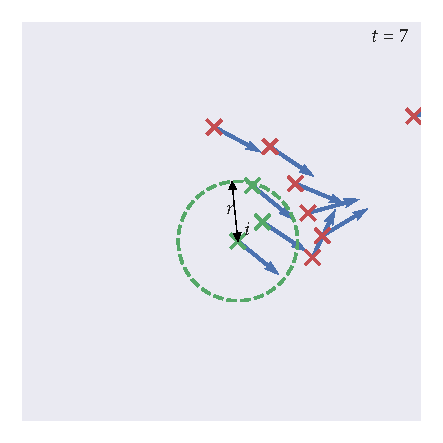
\includegraphics{vicsek_simulation_7.pdf}
    \end{subfigure}%
    \begin{subfigure}[b]{0.5\textwidth}
        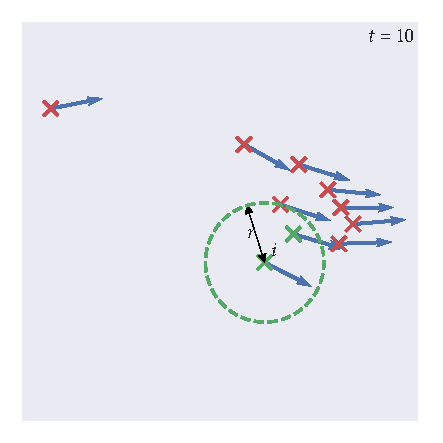
\includegraphics{vicsek_simulation_10.pdf}
    \end{subfigure}
    \caption{Visualisations from a simulation of the Vicsek model. At time $t=1$, $N=10$
        agents are assigned random positions within a square-cell of side length $L=1$.
        Initially, the directions of motion of individuals are realised from a
        $\mathcal{U}(-\pi, \pi)$ distribution. Between time steps agents move with speed
        $v=0.03$, and update directions according to \cref{eq:vicsek_update}, with
        $\eta=\pi/16$. The interaction zone of agent $i$ is illustrated throughout the
        simulation by a circle of radius $r$ centred at $\bm{x}_{i,t}$. The positions of
        neighbours within agent $i$'s interaction zone are visualised with a green cross.
        Individuals which lie outside of agent $i$'s interaction zone have their positions
        denoted by a red cross.}
\end{figure}

\section{Stuff I done thunk of whilst writing}

Although not specific to the Vicsek model, Vicsek introduced a measure of flock
alignment as 
\begin{equation}
    v_{a,t} = \frac{1}{Nv} \abs{\,\sum_{i=1}^N \bm{v}_{i,t}\,}.
\end{equation}


